\section{PNA-DNAdC5 structure 2017}

\subsection{Нормальное название}

Гибридный ДНК и-мотив*: аминоэтилпролил-ПНК** (pC5***) повышает стабильность и-мотива ДНК (dC5).

*"и" от "интеркалированный". И-мотив - это одна из структур, держащихся на водородных связях, которые, наравне с двухцепочечной структурой, могут образовывать нити ДНК (также РНК, ПНК).

**пептидно-нуклеиновая кислота - это как ДНК, только вместо дезоксирибозы вставлен пептид. В данном случае это аминоэтилпролил.

***pC5 имеется в виду кусочек из 5 цитозинов в ПНК, которые соединяются водородными связями при образовании и-мотива. То же касательно dC5.

\subsection{Абстракт}

Этот отчет описывает синтез богатых цитозином последовательностей, а именно пентамеров цитозина в аминоэтилпролиловом ПНК, и их биофизическое исследование для формирования смешанных ДНК-аэпПНК и-мотивных комплексов с пентамерами цитозина в кислотной среде.  Приведенные здесь исследования кругового дихроизма (КД), облучения в УФ, ЯМР, электроспрей масс-спектрометрии подтверждают образование стабильных гибридных ДНК-аэпПНК и-мотивов в кислотной среде. Следовательно, аэп-ПНК цитозин-богатые последовательности могут рассматриваться как потенциальные агенты для стабилизации ДНК и-мотива в живом организме (in vivo).

\subsection{Картинки}

\begin{figure}[H]
	\centering
	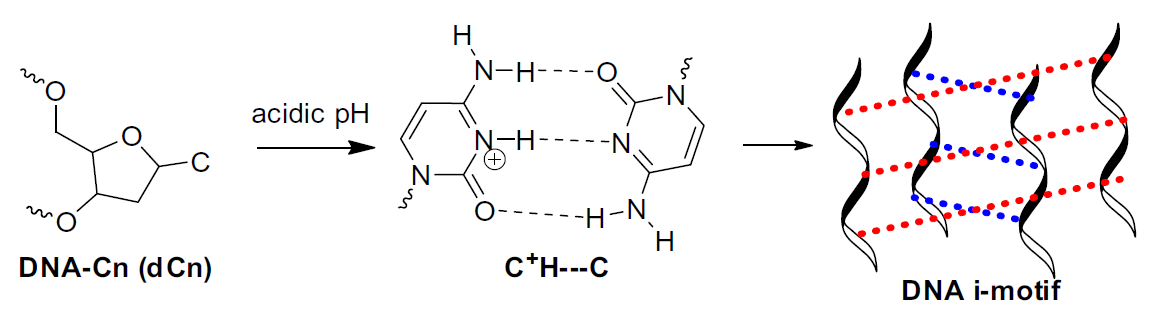
\includegraphics[width=0.5\linewidth]{2_1}
	\caption{Образование водородных связей между цитозинами ДНК в кислотной среде и формирование структуры под названием и-мотив.}
	\label{fig:2_1}
\end{figure}

\begin{figure}[H]
	\centering
	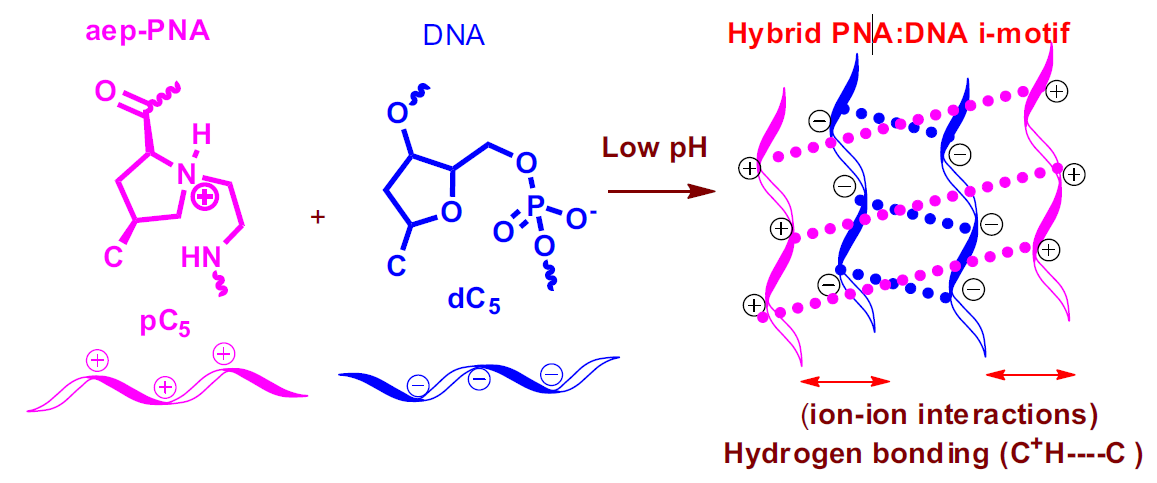
\includegraphics[width=0.5\linewidth]{2_2}
	\caption{Предполагаемая схема образования гибридного и-мотива.}
	\label{fig:2_2}
\end{figure}

Про картинку \ref{fig:2_2}. Что нужно заметить (про это спросили при обсуждении статьи): гибридный и-мотив в теории более устойчивый за счет того, что сцеплен не только водородными связями, но и электростатически.

\begin{figure}[H]
	\centering
	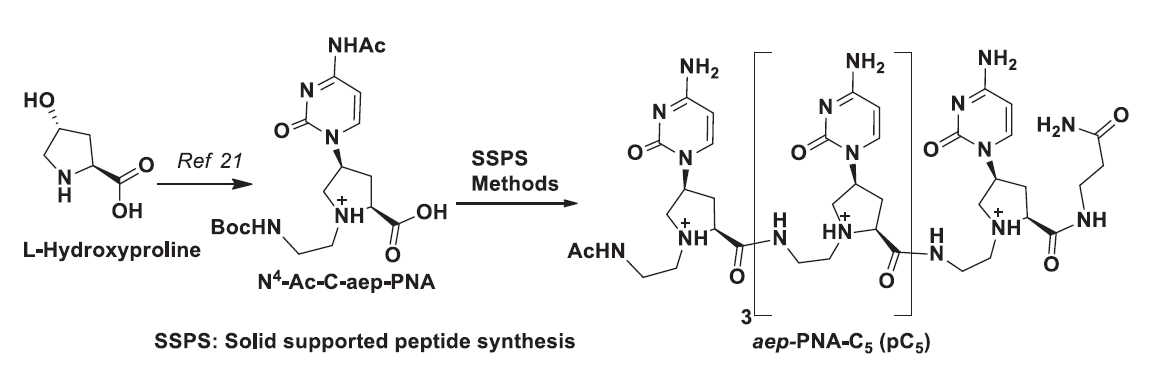
\includegraphics[width=0.5\linewidth]{2_3}
	\caption{Синтез цитозинового мономера аэп-ПНК и пентамера из цитозинов аэп-ПНК.}
	\label{fig:2_3}
\end{figure}

\begin{figure}[H]
	\centering
	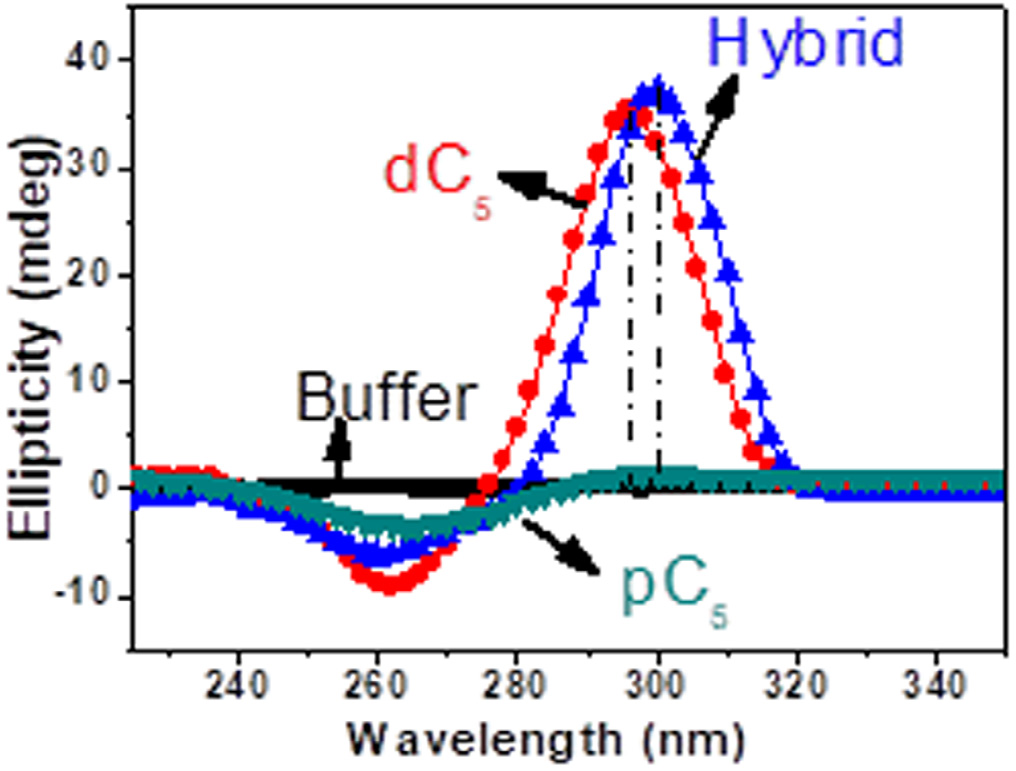
\includegraphics[width=0.5\linewidth]{2_4}
	\caption{КД-спектр (круговой дихроизм)  цитозин-пентамеров аэп-ПНК (45 мМ), ДНК (45 мМ), смеси аэп-ПНК и ДНК 1:1 (по 22.5 мМ каждый) при 10 градусах Цельсия,  рН 4.5.}
	\label{fig:2_4}
\end{figure}

Про картинку \ref{fig:2_4}. Что на графике: эллиптичность от длины волны.

Что нужно заметить: графики для гибрида и ДНК похожи, а вот ПНК принципиально отличается, так как имеет только минимум. Это означает, что тетраплексы (и-мотивы) из аэм-ПНК не образовывались за счет слишком сильного взаимного отталкивания заряженных нитей аэп-ПНК. Максимум на графике гибрида сдвинут относительно максимума для ДНК. В целом, график подтверждает образование гибридного тетраплекса в растворе ДНК с аэп-ПНК.

\begin{figure}[H]
	\centering
	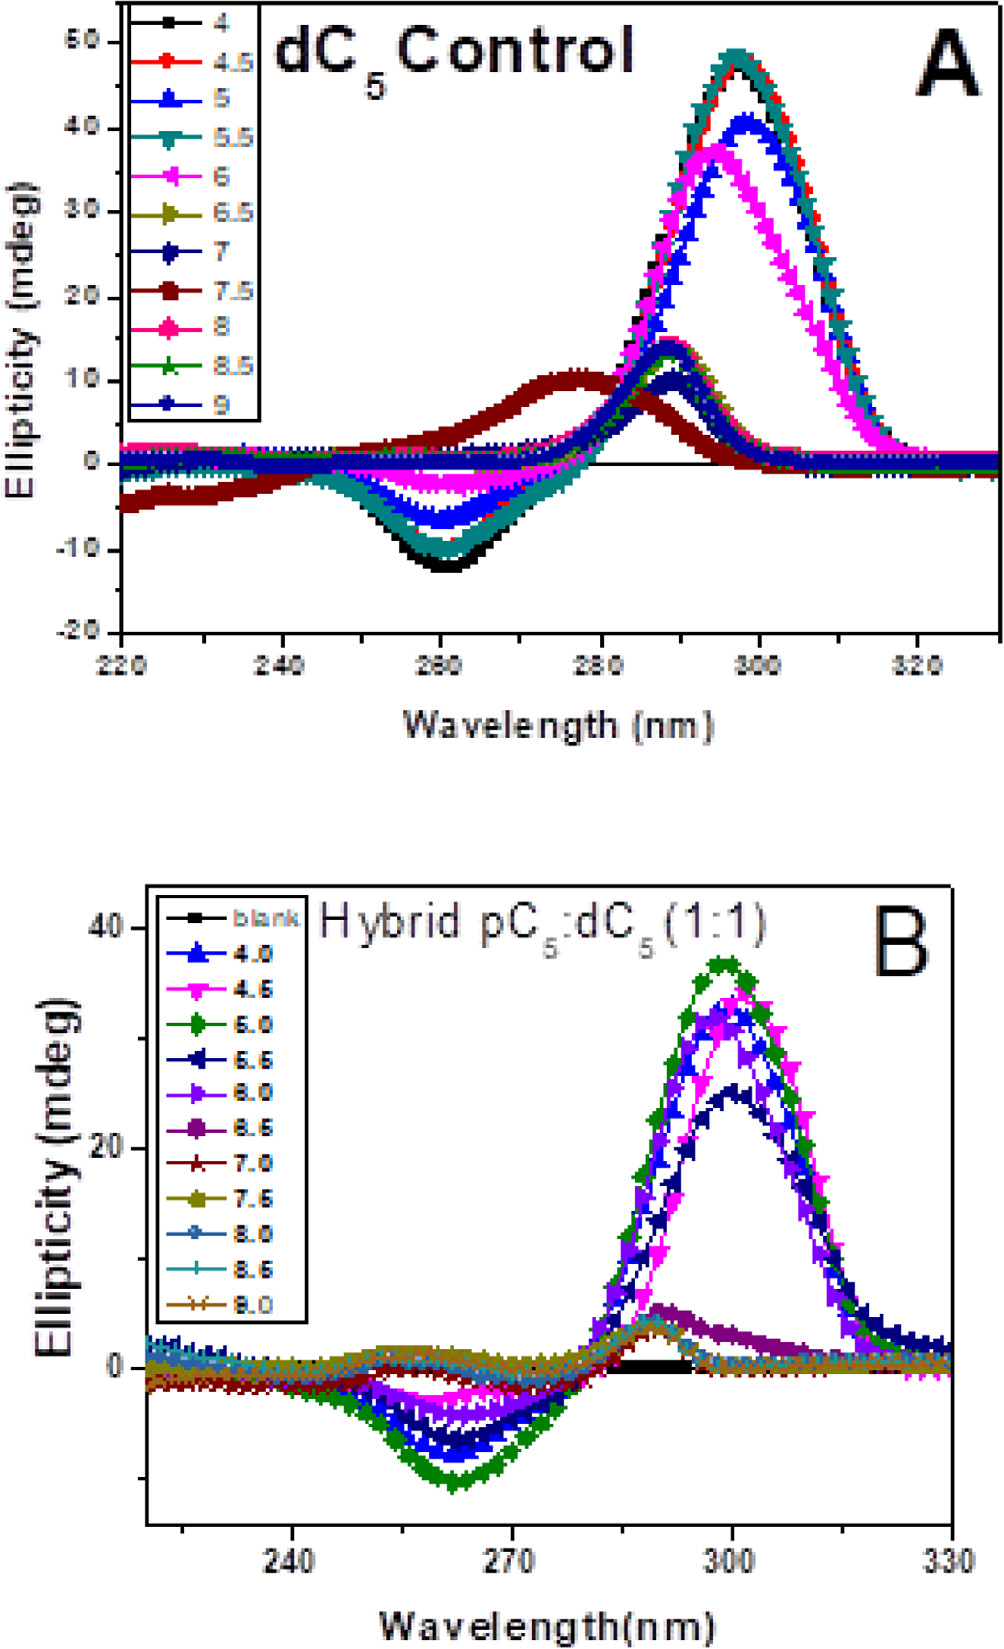
\includegraphics[width=0.5\linewidth]{2_5}
	\caption{КД-спектры при различных pH цитозин-пентамеров ДНК (45мМ) (на рис. А), смеси ДНК/аэп-ПНК (22.5 мМ каждый) (на рис. Б)}
	\label{fig:2_5}
\end{figure}

Про картинку \ref{fig:2_5}. На что обратить внимание: эти спектры снимали, чтобы выявить оптимальный pH для образования и-мотивов из ДНК и гибрида аэп-ПНК/ДНК соответственно. Оптимально оказалось 4-6 рН (кислая-слабокислая среда).

\begin{figure}[H]
	\centering
	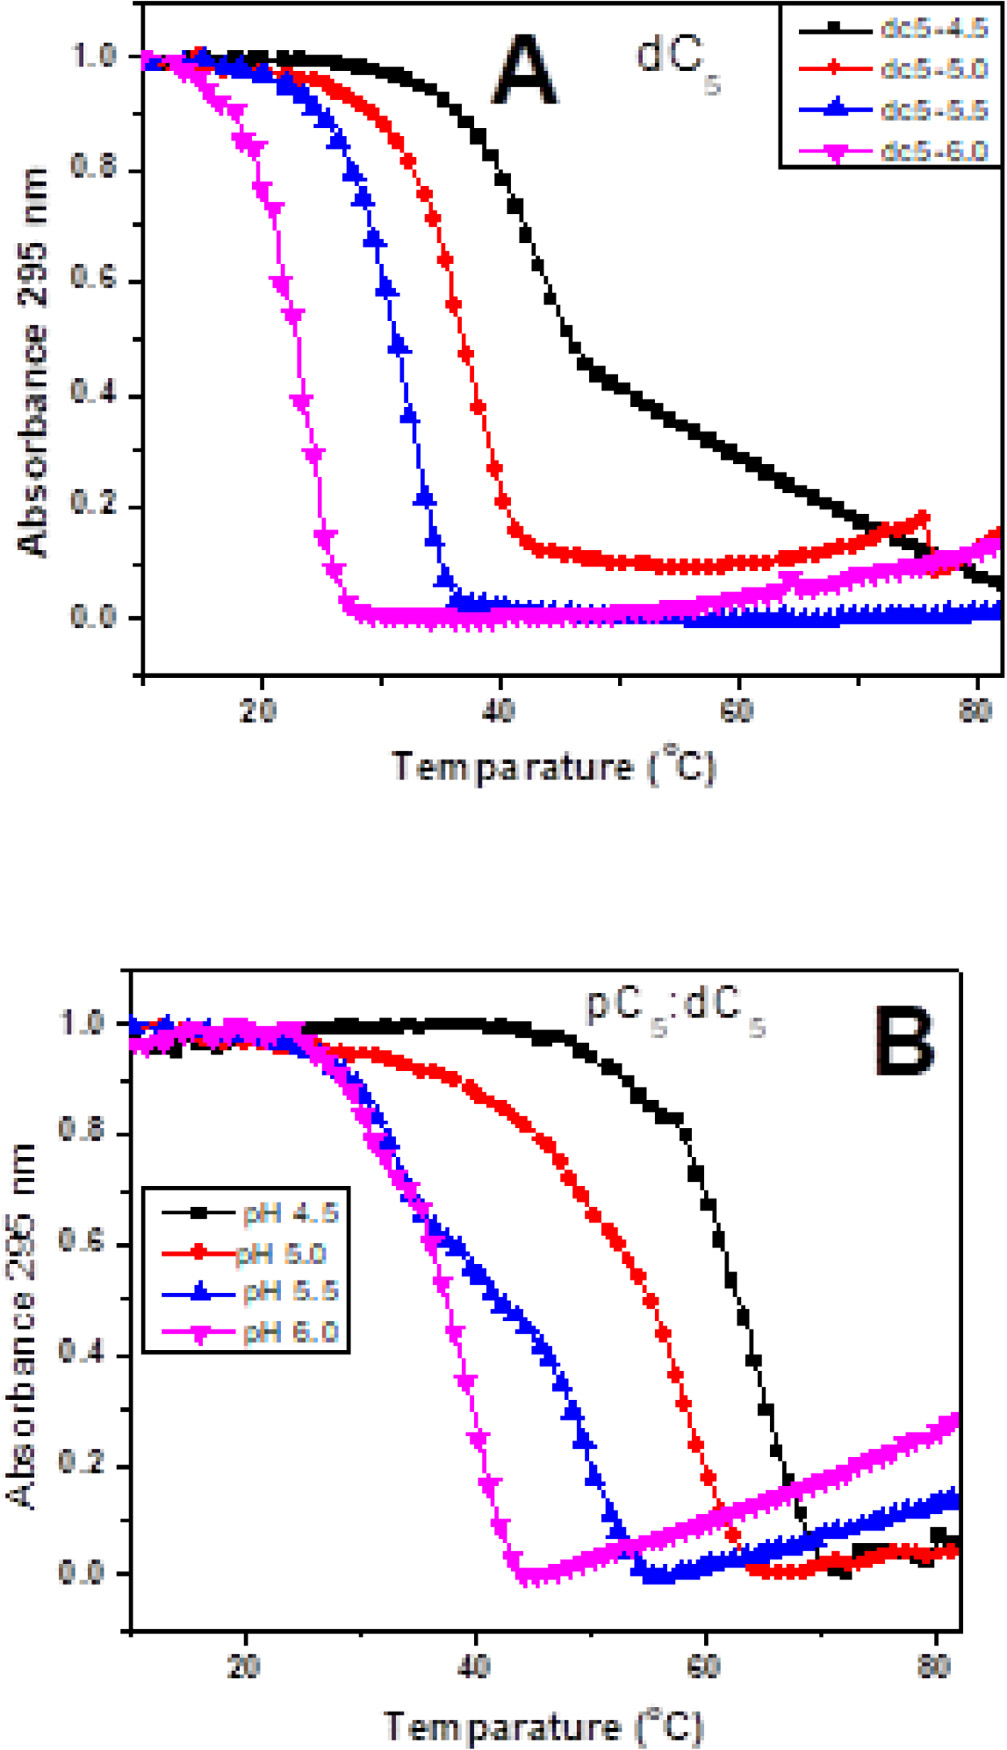
\includegraphics[width=0.5\linewidth]{2_6}
	\caption{Температурные профили плавления при различных pH при облучении УФ на длине волны 295 нм: цитозин-пентамеры ДНК (45.0 мМ), (B) цитозин пентамеры ДНК:аэп-ПНК (1:1) (22.5 мM каждый).}
	\label{fig:2_6}
\end{figure}

Про картинку \ref{fig:2_6}. На что обратить внимание: профили плавления на 300 нм в виде негативных сигмоид (общий вид кривых, которые мы видим на графиках) в целом характерны для тетраплексов ДНК (и-мотив - частный случай тетраплекса). Беря производную от данных кривых, можно обнаружить температуру плавления. Именно эти температуры выписаны в табл. 1.

\begin{figure}[H]
	\centering
	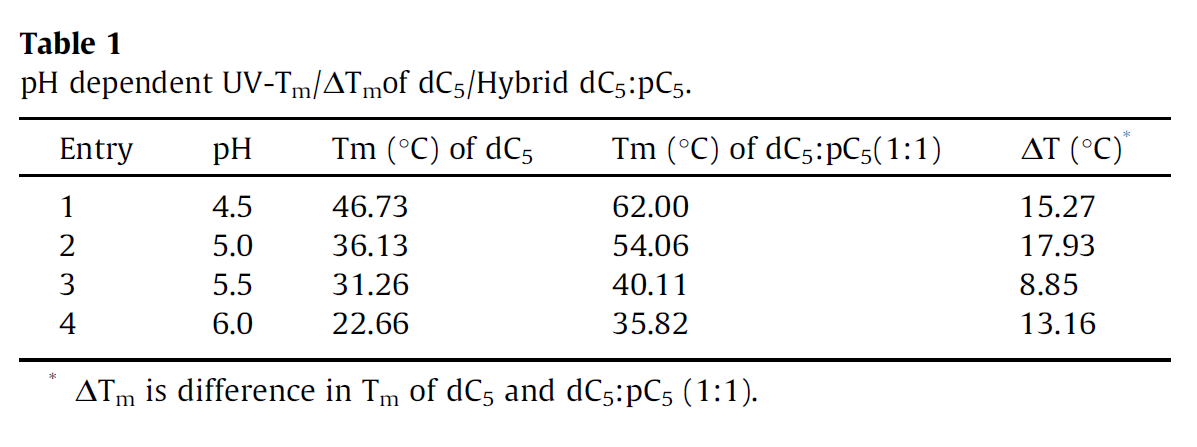
\includegraphics[width=0.5\linewidth]{2_7}
	\caption{Зависимость температуры плавления $T_m$ при облучении УФ  при различных pH для ДНК и для гибрида ДНК/аэп-ПНК}
	\label{fig:2_7}
\end{figure}

Про картинку \ref{fig:2_7}. Мы видим тенденцию, что при всех pH температура плавления для гибридного и-мотива выше, чем для ДНК и-мотива, что говорит о большей устойчивости гибрида.

\begin{figure}[H]
	\centering
	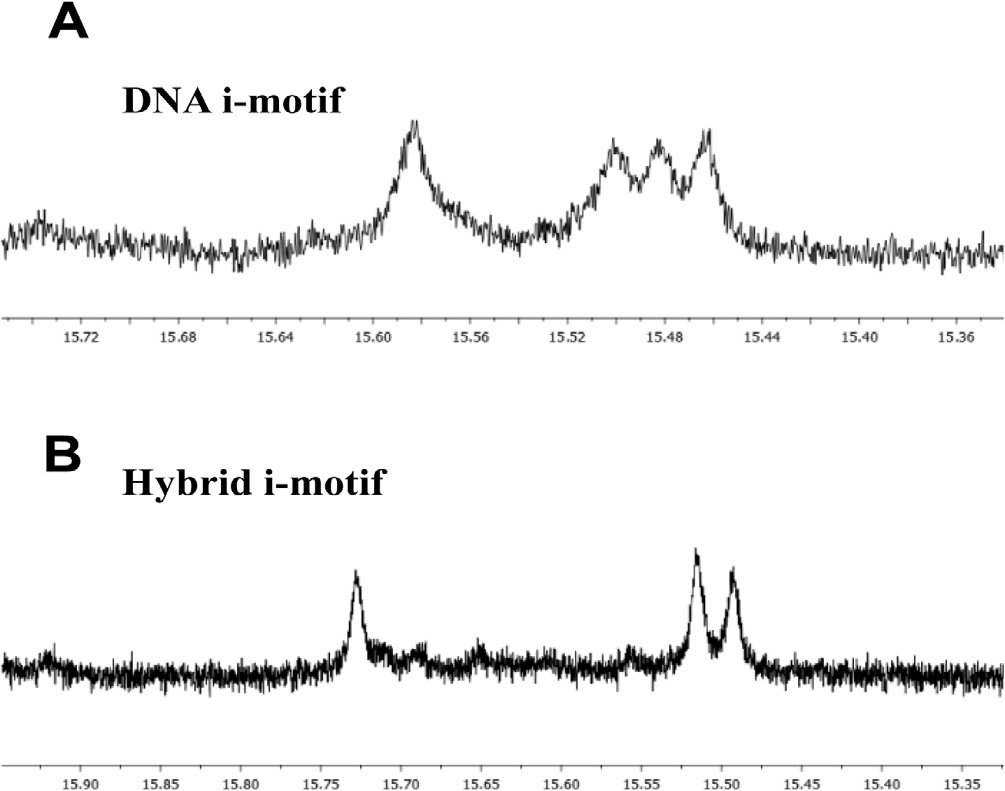
\includegraphics[width=0.5\linewidth]{2_8}
	\caption{Протонный магнитный резонанс водорода в связи H-N в протонированном цитозине при pH 4.5 при 25С (700 МГц) А) ДНК и-мотив (300 мМ), Б) гибрид ДНК/аэп-ПНК 1:1 (200 мМ каждый)}
	\label{fig:2_8}
\end{figure}

Про картинку \ref{fig:2_8}. Что по осям совершенно неясно :) Но форма графиков характерна для тетраплексных структур из ДНК

\begin{figure}[H]
	\centering
	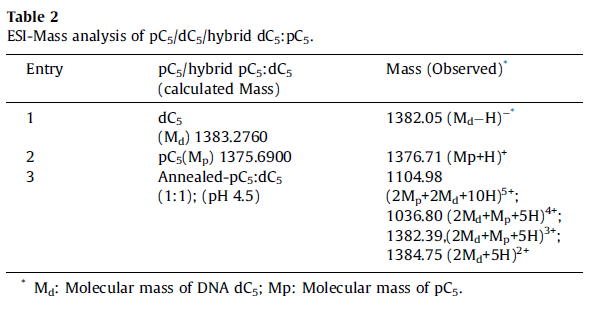
\includegraphics[width=0.5\linewidth]{2_9}
	\caption{Масс-спектрометрия электроспреевой ионизации цитозин-пентамеров аэп-ПНК, ДНК, гибрида ДНК/аэп-ПНК}
	\label{fig:2_9}
\end{figure}

Про картинку \ref{fig:2_9}. Собственно, есть три "входа" (соответственно, ПНК, ДНК и гибрид), обозначенных в первом столбце. Во втором - расчетная масса, в третьем - результаты измерений. Данные в третьем столбце - это интерпретация пиков с 7 картинки.

\begin{figure}[H]
	\centering
	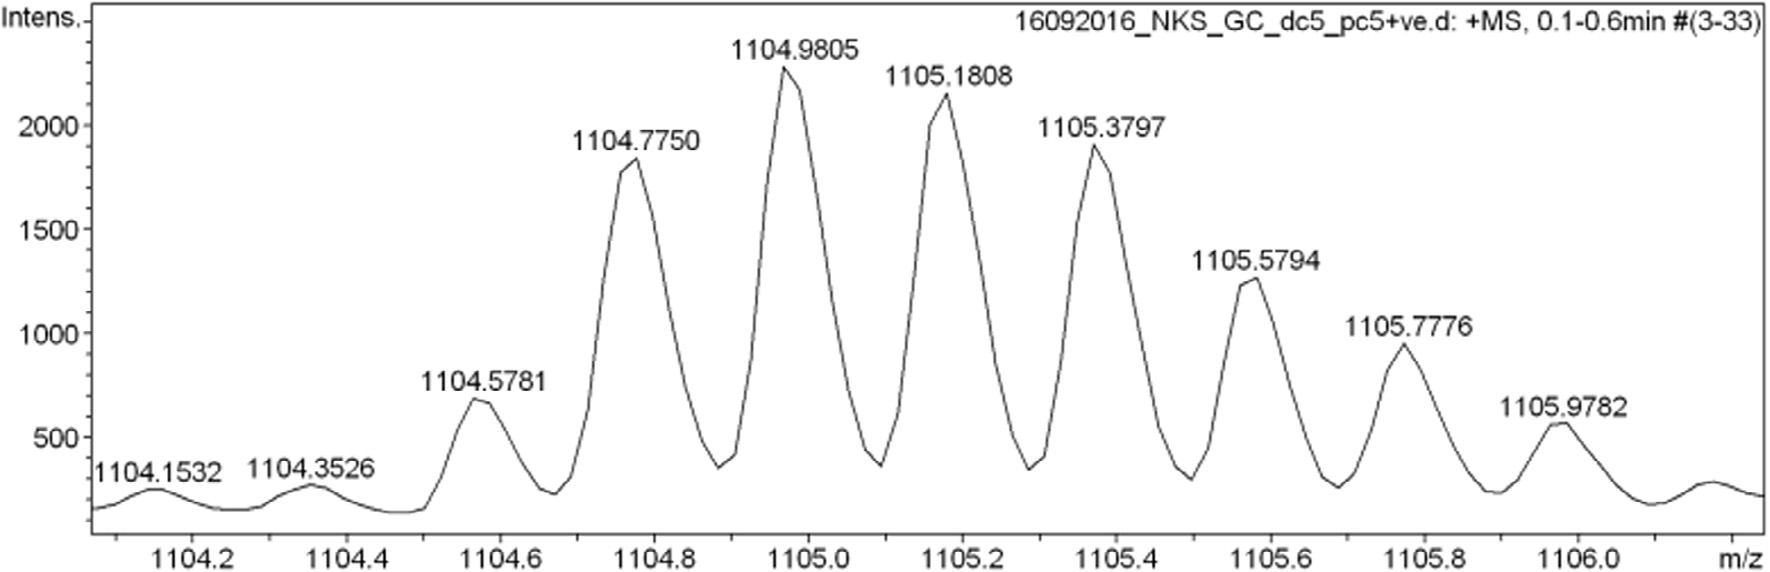
\includegraphics[width=0.7\linewidth]{2_10}
	\caption{Масс-спектр цитозин-пентамерного и-мотива ДНК/аэп-ПНК, полученный методом электроспреевой ионизации.}
	\label{fig:2_10}
\end{figure}

Про картинку \ref{fig:2_10}. Мы видим гребенку с шагом меньше 1 аем из-за изотопов.